% Title:
% 	Clean presentation template
% ----------------------
% Description:
% 	A clean, sans-serif presentation template.
%   This presentation uses custom fonts. You need to compile with xelatex,
%   and download Open Sans and Ubuntu Mono from:
%	
%	- https://www.fontsquirrel.com/fonts/open-sans
%	- https://www.fontsquirrel.com/fonts/ubuntu-mono
%
% Creator: Tommy O.

% -------------------------------------------------------------------------
% Setup
% -------------------------------------------------------------------------
\documentclass[12pt, aspectratio=149]{beamer}
% Options for aspectratio: 1610, 149, 54, 43 and 32, 169
\usepackage[utf8]{inputenc}
\usepackage[english]{babel}% Alternative: 'norsk'
\usepackage[expansion=false]{microtype}% Fixes to make typography better
\usecolortheme{beaver} % Decent options: beaver, rose, crane
%\useoutertheme{split}
%\useoutertheme[footline=authortitle]{miniframes}
\usepackage{listings}% To include source-code
\usepackage{booktabs}% Professional tables


\title{Presentation title}
\subtitle{Presentation subtitle}
\institute{Some institute}
\date{\today}
\author{Tommy O.}

% -------------------------------------------------------------------------
% Package imports
% -------------------------------------------------------------------------
\usepackage{etoolbox}
\usepackage{graphicx}
\usepackage{tikz}
\usepackage{amsmath}
\usepackage{amsthm}
\usepackage{amsfonts}
\usepackage{amssymb}
\usepackage{mathtools}
\usepackage{graphicx}
\usepackage{hyperref}
\usepackage{listings}
\usepackage[sharp]{easylist}
\usepackage{multicol}
\usepackage{tikz-cd}

% Set the math fonts - should be set before the others fonts, not sure why
\usepackage{sansmath} % Enables turning on sans-serif math mode
\sansmath % Enable sans-serif math for rest of document

% Set fonts to Open Sans and Ubuntu mono
\usefonttheme{professionalfonts}
\usepackage{fontspec}
\setmainfont{Open Sans}
\setsansfont{Open Sans}
\setmonofont{Ubuntu Mono}
\usefonttheme{serif}

%gets rid of bottom navigation bars
\setbeamertemplate{footline}[frame number]{}

%gets rid of bottom navigation symbols
\setbeamertemplate{navigation symbols}{}

% Set up colors to be used
\definecolor{titlecolor}{RGB}{31,119,180}
\definecolor{bggray}{RGB}{242,242,242}
\definecolor{bggraydark}{RGB}{217,217,217}

% Change the default colors

\setbeamercolor*{title}{bg=bggray,fg=titlecolor}
\AtBeginEnvironment{theorem}{%
	\setbeamercolor{block title}{fg=titlecolor, bg=bggraydark}
	\setbeamercolor{block body}{fg=black,bg=bggray}
}
\AtBeginEnvironment{proof}{%
	\setbeamercolor{block title}{bg=bggraydark}
	\setbeamercolor{block body}{fg=black,bg=bggray}
}
\AtBeginEnvironment{example}{%
	\setbeamercolor{block title example}{bg=bggraydark}
	\setbeamercolor{block body example}{fg=black,bg=bggray}
}
\AtBeginEnvironment{definition}{%
	\setbeamercolor{block title}{bg=bggraydark}
	\setbeamercolor{block body}{fg=black,bg=bggray}
}

\setbeamercolor{block title example}{bg=bggraydark}
\setbeamercolor{block body example}{fg=black,bg=bggray}
\setbeamercolor{block title}{bg=bggraydark}
\setbeamercolor{block body}{fg=black,bg=bggray}

\setbeamercolor{frametitle}{fg=titlecolor,bg=bggray}
\setbeamercolor{section in head/foot}{bg=black}
\setbeamercolor{author in head/foot}{bg=black}
\setbeamercolor{date in head/foot}{fg=titlecolor}

% Spacing for lsits
\newcommand{\listSpace}{0.2em}

% Theorems, equations, definitions setup
\theoremstyle{plain}

% Slides for sections
\AtBeginSection[]{
	\begin{frame}
		\vfill
		\centering
		\begin{beamercolorbox}[sep=8pt,center,shadow=false,rounded=false]{title}
			\usebeamerfont{title}\insertsectionhead\par%
		\end{beamercolorbox}
		\vfill
	\end{frame}
}

% -------------------------------------------------------------------------
% Document start
% -------------------------------------------------------------------------
\begin{document}
\maketitle
  
\begin{frame}{Table of contents}
	\tableofcontents
\end{frame}

% -------------------------------------------------------------------------
\section{First section}
\begin{frame}[fragile, t]{A slide with bullet points}
	\begin{easylist}[itemize]
		\ListProperties(Space=\listSpace, Space*=\listSpace)
		# Represent Abelian groups on the computer
		# Compute on Abelian groups
		# Solve equations, factor group homomorphisms
	\end{easylist}
\end{frame}

\begin{frame}[fragile, t]{A slide with a theorem and a proof.}
\begin{theorem}[Integral]
	\begin{equation*}
		\oint_\Gamma \mathbf{F}\, \cdot\, d{\mathbf{\Gamma}}  = \iint_S \nabla\times\mathbf{F}\, \cdot\, d\mathbf{S} 
	\end{equation*}
\end{theorem}
\begin{proof}
Here's the proof, if $a \to b$, then $\int_{a}^{b} \sum_i^n k^i$.
\end{proof}
\end{frame}

\begin{frame}[fragile, t]{A slide with two columns}
\begin{columns}
\begin{column}{0.5\textwidth}
	\begin{easylist}[itemize]
		\ListProperties(Space=\listSpace, Space*=\listSpace)
		# Represent Abelian groups
		# Compute on Abelian
		# Solve equations \footnotemark
	\end{easylist}
\end{column}
\begin{column}{0.5\textwidth}
    \begin{center}
     
\includegraphics[width=0.5\textwidth]{figs/UiB_logo.pdf}
     \end{center}
\end{column}
\end{columns}
\footnotetext{Often useful.}
\end{frame}

% -------------------------------------------------------------------------
\section{Second section}
\begin{frame}[fragile, t]{A slide with blocks}
	\begin{block}{title of the bloc}
	\begin{equation*}
	\left. \operatorname{div} \mathbf{F} \right|_p = \lim_{V \rightarrow \{p\}} \iint_{S(V)} \frac{\mathbf{F}\cdot\mathbf{\hat n}}{|V|} \, dS,
	\end{equation*}
	\end{block}
	
	\begin{exampleblock}{title of the bloc}
	$$\nabla r(x) = \frac{2}{x^* x} ( A x - r(x) x ) $$
	\end{exampleblock}
\end{frame}

% -------------------------------------------------------------------------
\section{Third section}
\begin{frame}[fragile, t]{A slide using pause}
	\begin{easylist}[itemize]
		\ListProperties(Space=\listSpace, Space*=\listSpace)
		# Represent Abelian groups on the computer \pause
		# Compute on Abelian groups \pause
		# Solve equations, factor group homomorphisms 
	\end{easylist}
\end{frame}

\begin{frame}[fragile, t]{A final figure}
	\begin{figure}
		\centering
		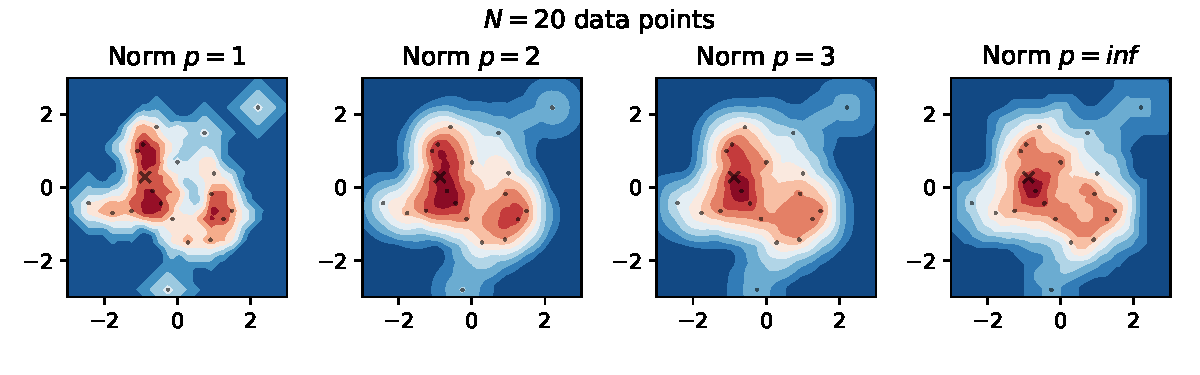
\includegraphics[width=1\linewidth]{figs/kde_example}
		\caption{Kernel density estimation.}
		\label{fig:kde_example}
	\end{figure}
\end{frame}


\end{document}
